% Created 2013-12-20 金 04:52
\documentclass[12pt]{jsarticle}
\usepackage[dvipdfmx]{graphicx}
\usepackage{comment}
%\usepackage{setspace}
%%\date{\today}
%\title{}
\textheight = 25truecm
\textwidth = 18truecm
\topmargin = -1.5truecm
\oddsidemargin = -1truecm
\evensidemargin = -1truecm
\marginparwidth = -1truecm
\def\theenumii{\Alph{enumii}}
\def\theenumiii{\alph{enumiii}}
\def\labelenumi{(\theenumi)}
\def\labelenumiii{(\theenumiii)}
%\setstretch{0.9}
\begin{document}

%\maketitle
%\tableofcontents

\begin{center}
%%%%%%%%%%%%%%%%%%%%%%%%%%%%%%%%%%%%%%%
%%%タイトル                         %%%
%%%%%%%%%%%%%%%%%%%%%%%%%%%%%%%%%%%%%%%
{\LARGE 共有メモリからデータを取得する割り込みハンドラの実行}
\end{center}

\begin{flushright}
  2014/9/30\\
  藤田将輝
\end{flushright}
%%%%%%%%%%%%%%%%%%1章%%%%%%%%%%%%%%%%%%%
\section{はじめに}

割り込み元OSから共有メモリにデータを格納し,IPIを送信すると割り込み先OSで割り込みハンドラが動作し,共有メモリからデータを取得
できることを確認した.
本資料ではこの流れを示す.

\section{割り込みハンドラが動作するまでの流れ}
割り込み元OSで共有メモリにデータを格納してから割り込み先OSで割り込みハンドラが動作し,共有メモリから
データを取得するまでの流れを図1に示し,以下で説明する.
\begin{enumerate}
\item AP2が割り込み先OSへ,コア1のベクタ表に割り込みハンドラを登録するシステムコールを発行する.
\item システムコールにより,割り込み先OSがコア1のベクタ表に割り込みハンドラを登録する.
\item AP1が割り込み元OSへ共有メモリにデータを格納するシステムコールを発行する.
\item システムコールにより,割り込み元OSが「fujita」という文字列を格納した配列を共有メモリに格納する.
\item AP0 が割り込み元OSへIPIを送信するシステムコールを発行する.
\item システムコールにより,割り込み元OSがコア0へIPIの送信要求を行う.
\item コア0がコア1へIPIを送信する.
\item 割り込み先OSの占有しているコア1がIPIを受信し,割り込みハンドラが動作する.
\item 割り込みハンドラにより,割り込み先OSが共有メモリから「fujita」という文字列を格納した配列を取得する.
\end{enumerate}



\begin{figure}[t]
\begin{center}
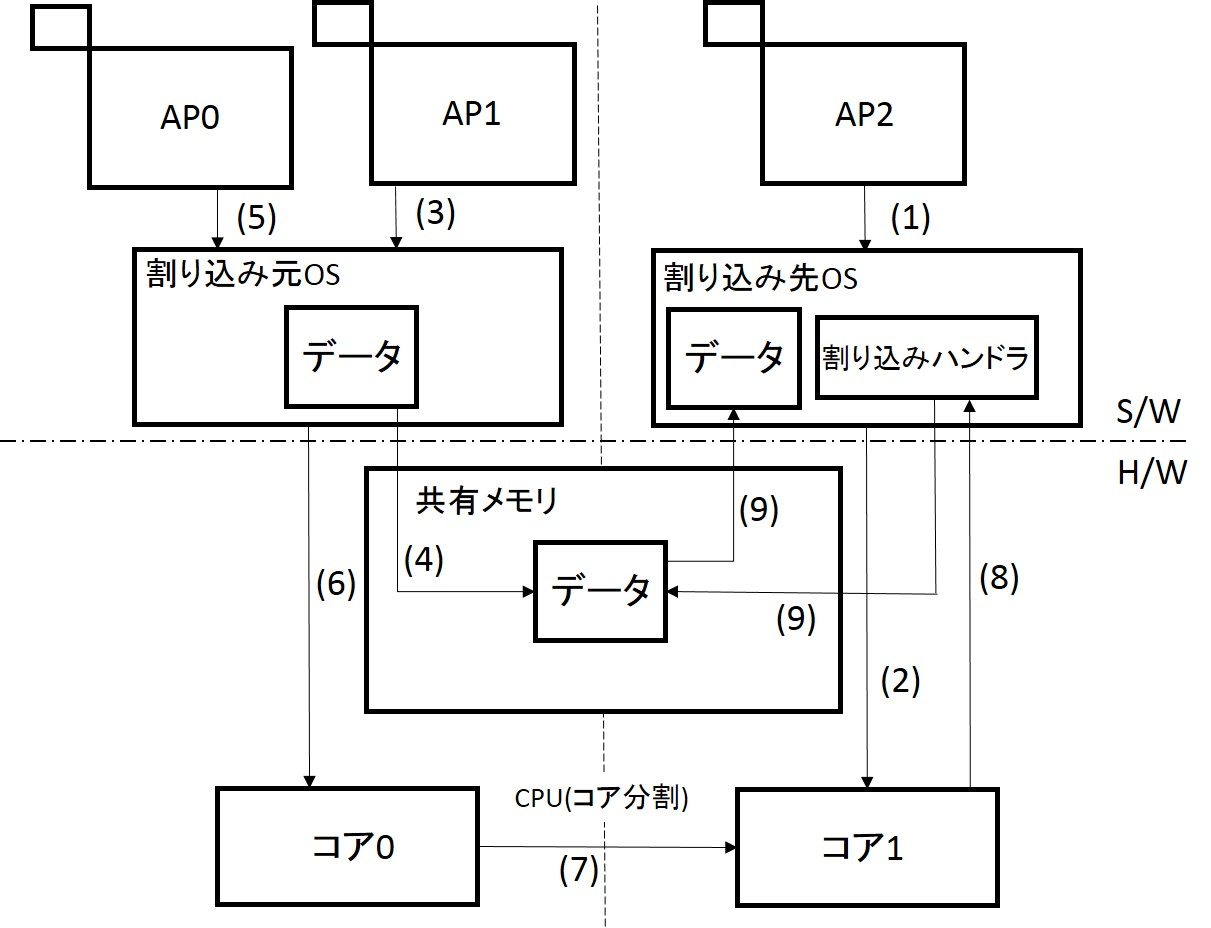
\includegraphics[height=8.0cm]{./fig1.jpg}
\caption{割り込みハンドラ動作までの流れ}
\label{fig:up}
\end{center}
\end{figure}


\section{使用したシステムコール}
\subsection{割り込みハンドラの登録}
割り込みハンドラの登録に使用したシステムコールについて以下に示す.
\begin{itemize}
\item [【形式】] asmlinkage int request\_ipi\_irq(int vector)
\item [【引数】] int vector: ベクタ番号
\item [【戻り値】] 成功:割り込みハンドラを登録したIRQ番号\\失敗:-1
\item [【機能】] 登録可能なIRQ番号irqを探し,irqに割り込みハンドラfujita\_ipi\_handlerを登録する.
その後,各コアのベクタ表vector\_irqのベクタ番号vectorのエントリにirqを登録する.
\end{itemize}
\subsection{共有メモリへのデータの格納}
共有メモリへのデータの格納に使用したシステムコールについて以下に示す.

\begin{itemize}
\item [【形式】] extern int sys\_mem\_test(void)
\item [【引数】] なし
\item [【戻り値】] 成功:1\\失敗:0以外
\item [【機能】] Mintの共有メモリに「fujita」という文字列を格納した配列を格納する機能を持つ.
今回の実験では0x1000020に「fujita」という文字列を格納した配列を格納した.
\end{itemize}
\subsection{IPIの送信}
IPIを送信するシステムコールについて以下に示す.
\begin{itemize}
\item [【形式】] asmlinkage void send\_yamamoto\_ipi(int core\_id, int vector, int n, int interval)
\item [【引数】] int core\_id:IPI送信先のコアID\\int vector:ベクタ番号\\int n:IPI送信回数\\int interval:IPI送信間隔
\item [【戻り値】] なし
\item [【機能】] core\_idのコアIDを持つコアへベクタ番号vectorの割り込みハンドラを実行させるIPIをn回連続で送信する.この際,IPIの送信間隔はintervalである.
\end{itemize}
\section{割り込みハンドラ}
登録した割り込みハンドラについて以下に示す.
\begin{itemize}
\item [【形式】] irqreturn\_t fujita\_ipi\_handler(int irq, void *dev\_id)
\item [【引数】] int irq:割り込みハンドラを登録するIRQ番号\\void *dev\_id:デバイスID
\item [【戻り値】] var配列のcpu要素
\item [【機能】] Mintの共有メモリからbufferに文字列を取得し,表示する.
\end{itemize}

\section{おわりに}
本資料では割り込み元OSで共有メモリにデータを格納し,割り込み先OSにIPIを送信後,割り込みハンドラによって
共有メモリからデータを取得する流れを示した.
今後はNICドライバの割り込み処理に必要なパケットの構造の調査とNICドライバの改変すべき箇所の調査を行い,実装する.

\end{document}
